\documentclass[tikz,border=8pt]{standalone}
% Shared look for every TikZ diagram. Load with % Shared look for every TikZ diagram. Load with % Shared look for every TikZ diagram. Load with \input{../../tools/tikz-style.tex}
\usepackage[T1]{fontenc}
\usepackage{lmodern}
\renewcommand{\sfdefault}{lmr}  % diagrams use the same serif as the text
\usetikzlibrary{arrows.meta, positioning, shapes.geometric, calc, fit, backgrounds}
\definecolor{cblue}{HTML}{4C78A8}
\definecolor{corange}{HTML}{F58518}
\definecolor{cgreen}{HTML}{54A24B}
\definecolor{cred}{HTML}{E45756}
\definecolor{cpurple}{HTML}{B279A2}
\definecolor{cgrey}{HTML}{6B6B6B}
\tikzset{
  every picture/.style={font=\sffamily, line width=1.2pt},
  box/.style={draw=#1, fill=#1!12, rounded corners=4pt, align=center, inner sep=7pt, minimum height=1.1cm},
  box/.default=cgrey,
  arrow/.style={-{Stealth[length=3mm]}, draw=cgrey, line width=1.4pt},
  title/.style={font=\sffamily\bfseries\Large},
  note/.style={font=\sffamily\small, text=cgrey, align=center},
}
\AtBeginDocument{\hyphenpenalty=10000 \exhyphenpenalty=10000}

\usepackage[T1]{fontenc}
\usepackage{lmodern}
\renewcommand{\sfdefault}{lmr}  % diagrams use the same serif as the text
\usetikzlibrary{arrows.meta, positioning, shapes.geometric, calc, fit, backgrounds}
\definecolor{cblue}{HTML}{4C78A8}
\definecolor{corange}{HTML}{F58518}
\definecolor{cgreen}{HTML}{54A24B}
\definecolor{cred}{HTML}{E45756}
\definecolor{cpurple}{HTML}{B279A2}
\definecolor{cgrey}{HTML}{6B6B6B}
\tikzset{
  every picture/.style={font=\sffamily, line width=1.2pt},
  box/.style={draw=#1, fill=#1!12, rounded corners=4pt, align=center, inner sep=7pt, minimum height=1.1cm},
  box/.default=cgrey,
  arrow/.style={-{Stealth[length=3mm]}, draw=cgrey, line width=1.4pt},
  title/.style={font=\sffamily\bfseries\Large},
  note/.style={font=\sffamily\small, text=cgrey, align=center},
}
\AtBeginDocument{\hyphenpenalty=10000 \exhyphenpenalty=10000}

\usepackage[T1]{fontenc}
\usepackage{lmodern}
\renewcommand{\sfdefault}{lmr}  % diagrams use the same serif as the text
\usetikzlibrary{arrows.meta, positioning, shapes.geometric, calc, fit, backgrounds}
\definecolor{cblue}{HTML}{4C78A8}
\definecolor{corange}{HTML}{F58518}
\definecolor{cgreen}{HTML}{54A24B}
\definecolor{cred}{HTML}{E45756}
\definecolor{cpurple}{HTML}{B279A2}
\definecolor{cgrey}{HTML}{6B6B6B}
\tikzset{
  every picture/.style={font=\sffamily, line width=1.2pt},
  box/.style={draw=#1, fill=#1!12, rounded corners=4pt, align=center, inner sep=7pt, minimum height=1.1cm},
  box/.default=cgrey,
  arrow/.style={-{Stealth[length=3mm]}, draw=cgrey, line width=1.4pt},
  title/.style={font=\sffamily\bfseries\Large},
  note/.style={font=\sffamily\small, text=cgrey, align=center},
}
\AtBeginDocument{\hyphenpenalty=10000 \exhyphenpenalty=10000}

\begin{document}
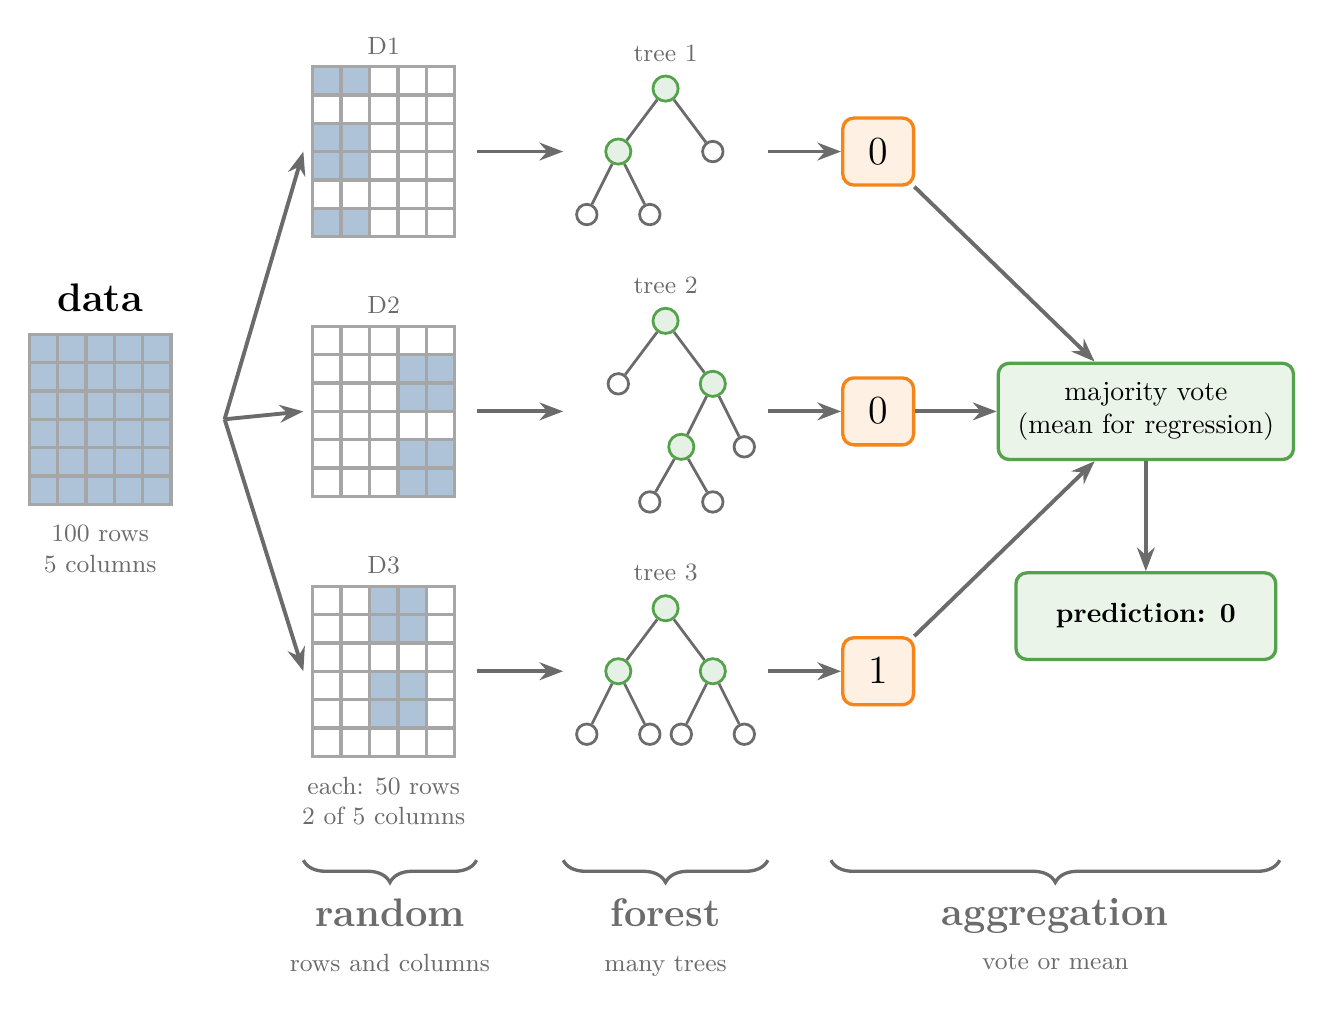
\begin{tikzpicture}[cell/.style={draw=cgrey!60, minimum size=0.36cm, inner sep=0pt},
  nd/.style={circle, draw=cgreen, fill=cgreen!15, minimum size=0.32cm, inner sep=0pt, line width=1pt},
  lf/.style={circle, draw=cgrey, fill=white, minimum size=0.26cm, inner sep=0pt, line width=1pt},
  edge/.style={draw=cgrey, line width=1pt},
  v/.style={box=corange, minimum width=0.9cm, minimum height=0.85cm, font=\sffamily\Large},
  o/.style={box=cgreen, minimum width=3.3cm}]
  % \grid{x}{y}{rows used}{cols used}: a mini table of 6 rows x 5 columns, blue = what this tree sees
  \newcommand{\grid}[4]{
    \begin{scope}[shift={(#1,#2)}]
      \foreach \r in {0,...,5} \foreach \c in {0,...,4} {
        \def\fillc{white}
        \foreach \rr in {#3} {\ifnum\r=\rr \foreach \cc in {#4} {\ifnum\c=\cc \xdef\fillc{cblue!45}\fi}\fi}
        \node[cell, fill=\fillc] at (\c*0.36,-\r*0.36) {};
        \gdef\fillc{white}
      }
    \end{scope}}
  % full data
  \grid{0}{1.0}{0,1,2,3,4,5}{0,1,2,3,4}
  \node[title] at (0.72,1.65) {data};
  \node[note] at (0.72,-1.55) {100 rows\\5 columns};
  % three subsets (columns as in the Notebook: col1+col2, col4+col5, col3+col4)
  \grid{3.6}{4.4}{0,2,3,5}{0,1}
  \grid{3.6}{1.1}{1,2,4,5}{3,4}
  \grid{3.6}{-2.2}{0,1,3,4}{2,3}
  \foreach \i/\y in {1/4.4, 2/1.1, 3/-2.2} \node[note, anchor=south] at (4.32,\y+0.2) {D\i};
  \node[note] at (4.32,-4.75) {each: 50 rows\\2 of 5 columns};
  \foreach \y in {3.5,0.2,-3.1} \draw[arrow] (2.3,0.1) -- (3.3,\y);
  % three different trees
  \begin{scope}[shift={(7.9,4.3)}]
    \node[nd] (a) at (0,0) {}; \node[nd] (b) at (-0.6,-0.8) {}; \node[lf] (c) at (0.6,-0.8) {};
    \node[lf] (d) at (-1.0,-1.6) {}; \node[lf] (e) at (-0.2,-1.6) {};
    \draw[edge] (a)--(b) (a)--(c) (b)--(d) (b)--(e);
  \end{scope}
  \begin{scope}[shift={(7.9,1.35)}]
    \node[nd] (a) at (0,0) {}; \node[lf] (b) at (-0.6,-0.8) {}; \node[nd] (c) at (0.6,-0.8) {};
    \node[nd] (d) at (0.2,-1.6) {}; \node[lf] (e) at (1.0,-1.6) {}; \node[lf] (f) at (-0.2,-2.3) {}; \node[lf] (g) at (0.6,-2.3) {};
    \draw[edge] (a)--(b) (a)--(c) (c)--(d) (c)--(e) (d)--(f) (d)--(g);
  \end{scope}
  \begin{scope}[shift={(7.9,-2.3)}]
    \node[nd] (a) at (0,0) {}; \node[nd] (b) at (-0.6,-0.8) {}; \node[nd] (c) at (0.6,-0.8) {};
    \node[lf] (d) at (-1.0,-1.6) {}; \node[lf] (e) at (-0.2,-1.6) {}; \node[lf] (f) at (0.2,-1.6) {}; \node[lf] (g) at (1.0,-1.6) {};
    \draw[edge] (a)--(b) (a)--(c) (b)--(d) (b)--(e) (c)--(f) (c)--(g);
  \end{scope}
  \foreach \i/\y/\t in {1/3.5/4.3, 2/0.2/1.35, 3/-3.1/-2.3} {
    \draw[arrow] (5.5,\y) -- (6.6,\y);
    \node[note] at (7.9,\t+0.45) {tree \i};
  }
  % votes and the majority
  \foreach \i/\y/\v in {1/3.5/0, 2/0.2/0, 3/-3.1/1} {\node[v] (p\i) at (10.6,\y) {\v}; \draw[arrow] (9.2,\y) -- (p\i);}
  \node[o] (agg) at (14.0,0.2) {majority vote\\(mean for regression)};
  \foreach \i in {1,2,3} \draw[arrow] (p\i) -- (agg);
  \node[o, font=\sffamily\bfseries] (out) at (14.0,-2.4) {prediction: 0};
  \draw[arrow] (agg) -- (out);
  % what the two words mean
  \draw[decorate, decoration={brace, amplitude=8pt, mirror}, cgrey, line width=1.2pt] (3.3,-5.5) -- (5.5,-5.5)
     node[midway, below=10pt, title, align=center] {random\\[-2pt]{\normalfont\small rows and columns}};
  \draw[decorate, decoration={brace, amplitude=8pt, mirror}, cgrey, line width=1.2pt] (6.6,-5.5) -- (9.2,-5.5)
     node[midway, below=10pt, title, align=center] {forest\\[-2pt]{\normalfont\small many trees}};
  \draw[decorate, decoration={brace, amplitude=8pt, mirror}, cgrey, line width=1.2pt] (10.0,-5.5) -- (15.7,-5.5)
     node[midway, below=10pt, title, align=center] {aggregation\\[-2pt]{\normalfont\small vote or mean}};
\end{tikzpicture}
\end{document}
